\newcommand{\institut}{Institut f\"ur Telekommunikationssysteme}
\newcommand{\fachgebiet}{Nachrichten\"ubertragung}
\newcommand{\veranstaltung}{Praktikum Nachrichten\"ubertragung}
\newcommand{\pdfautor}{Dirk Babendererde (321 836), Thomas Kapa (325 219)}
\newcommand{\autor}{Dirk Babendererde (321 836)\\ Thomas Kapa (325 219)}
\newcommand{\gruppe}{Gruppe:}
\newcommand{\betreuer}{Betreuer: Lieven Lange}


\newcommand{\pdftitle}{Nachrichtenuebertragung\ Praktikum\ 03}
\newcommand{\prototitle}{Praktikum 03 \\ Statistische Nachrichtentheorie}

\input{../../packages/tu_header_9}
%\begin{document}


%     \lstinputlisting{./praktikum6.sce}

%---------------------------------------------------------------------
%---------------------------------------------------------------------
%---------------------------------------------------------------------


\section{Vorbereitungsaufgaben}
\begin{quote}
    \hspace{-2em}
    \subsection{Herleitung der Spektren}
    \begin{quote}
        
        \subsubsection{Shape-Top-Abtastung}
        \begin{quote}
            
            
            \begin{equation*}
                \begin{split}
                    f_m (t)   &= f(t) \cdot \sqcap_{\alpha T} (t) \ast \delta_T (t) \\
                    F_m (j\omega) &= \frac{1}{2\pi} F (j\omega) \ast \left [ \alpha T \cdot si \left( \frac{\omega
                    \alpha T}{2} \right) \cdot \omega_T \cdot \delta_{\omega T} (\omega) \right] \\
                    &= \alpha \cdot F (j \omega) \ast \left ( si \left( \frac{\omega \alpha T}{2} \right)
                    \sum_{k=-\infty}^{\infty} \delta (\omega - k\omega_T) \right)\\
                    &= \alpha \cdot F (j \omega) \ast \sum_{k=-\infty}^{\infty} (si(k \pi \alpha) \cdot \delta (\omega -
                    k\omega_T))\\
                    &= \alpha \cdot \sum_{k=-\infty}^{\infty} \left [ si(k \pi \alpha) \cdot F (j(\omega - k\omega_T))
                    \right]\\
                    \label{eq:shape}
                \end{split}
            \end{equation*}
            
            
        \end{quote}
        
        \subsubsection{Flat-Top-Abtastung}
        \begin{quote}
            
            
            \begin{equation*}
                \begin{split}
                    f_m (t) &= [f (t) \cdot \delta_T (t)] \ast \sqcap_{\alpha T} (t)\\
                    F_m (j\omega) &= \left ( \frac{1}{2 \pi} F (j\omega) \ast \omega_T \cdot \delta_T (\omega) \right) \cdot
                    \alpha T \cdot si (\frac{\alpha \omega T}{2})\\
                    &= \alpha \cdot si \left( \frac{\omega \alpha T}{2} \right) \cdot \sum_{k=-\infty}^{\infty} F(j(\omega -
                    k\omega_T))\\
                    \label{eq:flat}
                \end{split}
            \end{equation*}
            
            
        \end{quote}
        
        
    \end{quote}
    
    
    \subsection{Skizzieren}
    \begin{quote}
        Zur übung das Spektrum folgenden Signals
        
        \begin{equation*}
        	\begin{split}
                f(t) = A \p cos(\frac{\omega_T}{5} t)
        	\end{split}
        \end{equation*}
        
        mit $\alpha = 0,5$ und $\omega_T =$ \SI{20}{\pi\ \kilo\hertz} Skizzieren.
        
        
        \begin{figure}[H]
        \centering\fbox{
            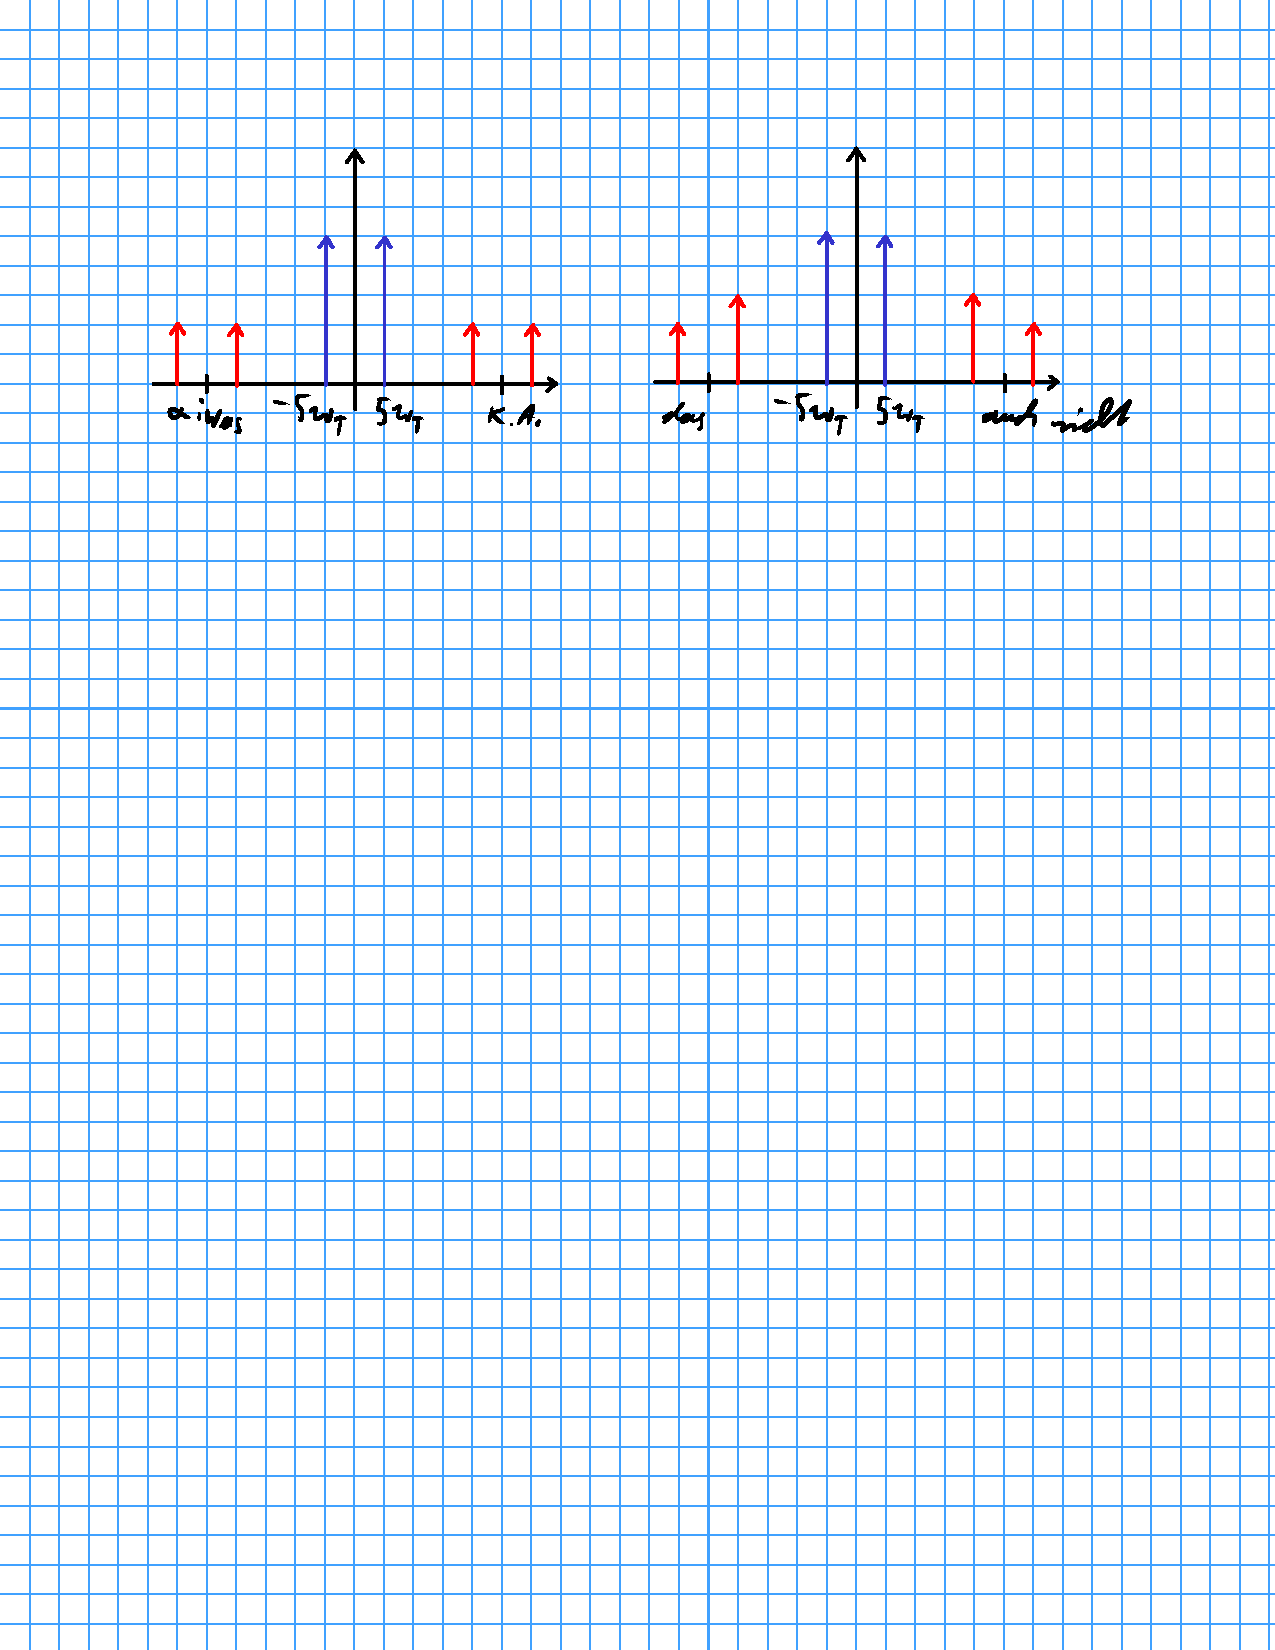
\includegraphics[scale=0.7, trim = 1cm 18cm 1cm 2cm, clip]{Bilder/skizze}}
                \caption{sampling Skizze}
                \label{fig:skizze}
        \end{figure}
        
        
    \end{quote}
    
    
    \subsection{MatLab-Simulation}
    \begin{quote}
        Um unsere Durchführungsergebnisse mit idealen Werten vergleichen zu können haben wir die Praktikumsaufgaben in
        Matlab simuliert.
    \end{quote}
    
    
    
    
    
    
\end{quote}

%--------------------------------------------------------------------
%--------------------------------------------------------------------


\section{Durchführung}
\begin{quote}
    
    
    \subsection{Labordurchführung}
    \begin{quote}
         Für die Signalausblendung (Shape-Top-Sampling) und die
     Signalverbreiterung (Flat-Top-Sampling) wird das Dual Analog Switch- Modul
     verwendet.
     Bei beiden Samplingvarianten wird auf den Eingang Control 1 ein
     unipolares Rechtecksignal mit einer Spannung von 0 bis 5 Volt, variabler
     Frequenz (10 und 20 Hz) und variablem Tastverhältnis (0,2 , 0,5 und 0,7)
     gelegt. Dieses wird vom Signalgenerator geliefert.
     Es sollen drei abzutastende Signale untersucht werden. Zum einen ein
     bipolares, mittelwertfreies Rechtecksignal mit einer Spitze-Spitze-Spannung von 4 Volt und einer
     Frequenz von 2 kHz, welches vom Master Signals Modul geliefert wird. Dafür
     wird der Ausgang 2 kHz DIGITAL verwendet. Dieser liefert allerdings ein
     Rechtecksignal mit der Spannung von 0 bis 5 Volt. Damit man das
     bipolare Signal erhält, wird das ADDER Modul verwendet. Das Rechtecksignal
     wird auf den Eingang B gegeben, wo das Signal mittels der Verstärkung von
     4/5 auf 0 bis 4 Volt eingestellt wird. Da der ADDER invertiert muss zuletzt
     nur noch ein Offset von 2 Volt mit Hilfe des Variable DC Moduls gegeben
     werden.\\
     \noindent\hspace*{4mm}% 
     Als zweites Signal soll das eben erstellte bipolare Rechtecksignal vor
     der Abtastung tiefpassgefiltert werden. Dazu wird das RC LPF Modul, also
     ein Tiefpass bestehend aus einem Kondensator und einer Spule, verwendet.
     Zum anderen soll ein 2 kHz Sinussignal abgetastet werden, welches ebenfalls
     dem Master Signals Modul entnommen werden kann.\\
     \noindent\hspace*{4mm}% 
     Bei der Signalausblendung wird das abzutastende Signal auf den Eingang
     IN1 gegeben und der Ausgang am Out abgegriffen. Damit wird
     ein Schalter geöffnet und geschlossen, was dazu führt, dass die Kontur
     des Signals im Abtastpuls mit übertragen wird (daher Shape-Top).\\
     Bei der Signalverbreiterung wird das Quellensignal noch zusätzlich vorher
     durch ein S/H-Glied, also ein Abtast- und Halteglied (S&H
     IN, S&H OUT) und von da aus in IN1 geführt. Dieses sorgt dafür, dass bei
     einem Abtastimpuls nur ein Wert durchgängig übertragen wird (daher
     Flat-Top).\\ 
     \noindent\hspace*{4mm}% 
     Zuletzt wird das Signal zur Rekonstruktion noch durch einen Tiefpassfilter
     mit variabler Grenzfrequenz geführt (TUNEABLE LPF IN/OUT).\\
     \noindent\hspace*{4mm}% 
     Für die Messungen wird das Abtastsignal sowohl in der Frequenz, als auch in
     dem Tastgrad, wie oben gegeben für Signalverbreiterung und
     Signalausblendung variiert. 
     Dabei kann man einige der Kombinationen auslassen. Da sich die
     Veränderungen von $\alpha$ bei 10 und 20 kHz ähnlich auswirken, wird im
     Versuch nur der Tastgrad für 20 kHz variiert.\\
     \noindent\hspace*{4mm}% 
     Im zweiten Teil soll ein
     Sprachsignal mit Signalausblendung oder Signalverbreiterung abgetastet werden. Dazu wird ein Mikrofon des SPEECH Modul genutzt und beim BUFFER Modul ein Kopfhörer angeschlossen.
    \end{quote}
    
    
    \subsection{Auswertung \& Theorie}
    \begin{quote}
        
        Im Labor haben wir dann folgende Messungen durchgefüht.
        
        \TODO{Thommy: wollen wir ne Tabelle? Neeeeiiiiiiin das sieht man dann
        doch an den Bildern}
        
        
        
        \subsubsection{änderung der Trägerfrequenz}
        \begin{quote}
            
            Der Theorie nach sollte das Signal, das mit einer höheren
            Frequenz abgestastet wird, auf Grund der Mehrzahl an Stützstellen
            auch besser rekonstruiert werden.
            Das reine Rechtecksignal sollte ein starkes Überschwingen zeigen, da
            es unendlich viele Frequenzanteile enthält und das Abtasttheorem für
            die großen Frequenzen nicht eingehlten werden kann.
            Das tiefpassgefilterte Rechtecksignal sollte aufgrund der
            entnommenen hohen Frequenzen weniger Überschwingen nach der rekonstruktion enthalten.
            Der nahezu reine Sinus sollte ziemlich gut rekonstruiert werden
            können, da er effektiv nur einen Frequenzanteil enthält.
            
            
            Man kann gut erkennen, dass die Filterung des Rechtecksignals vor
            der Abtastung eine Glättung des rekonstruierten Signals hervorruft.  
            die gemessenen Werte sehen so aus\\
            
            FIGURE\\
            \\
            
            
            verglichen mit den Simulierten werten\\
            
            FIGURE\\
            
            is das toll\\
        \end{quote}


        \subsubsection{änderung des \alpha }
        \begin{quote}
             
             Der Theorie nach sollte das Signal, welches mit einem größeren
             Tastgrad abgetastet wird auch eine höhere Amplitude im Spektrum und
             im rekonstruierten Signal haben, da wie in den Formeln
             \ref{eq:shape} und \ref{eq:flat} als Vorfaktor auftauchen. Für ein kleineres $\alpha$ sollte sich aber eine
             bessere Rekonstruktion des Ausgangssignals ergeben, da das
             Abtastsignal immer mehr einem für die Abtastung idealen
             Deltaimpuls ähnelt.
             Bei der Signalausblendung sollte das Basisband (k=0) um $\alpha$
             verringern. Alle anderen Bänder sollten sich noch zusätzlich um den
             Faktor $si(k\alpha\pi)$ verringern, was zu einer Verzerrung führt.
             Im Gegensatz dazu werden bei der Signalverbreiterung alle Bänder
             mit dem Faktor $si(\omega \alpha T/2)$ verzerrt. Da damit das
             Basisbandsignal ebenfalls verzerrt ist, kann das Signal auch mit
             einem idealen Tiefpass nicht wiedergewonnen werden.
             
             
             Wie man erkennen kann, ähnelt die Rekonstruktion der
             Signalausblendung eher dem Urspungssignal, was wie nach der Theorie
             erwartet an dem verzerrten Basisband bei der Signalverbreiterung
             liegt.
        \end{quote}

        
        
        
    \end{quote}
    
\end{quote}









% \begin{quote}
%     \lstinputlisting[
%         caption={Scilab-script},
%         label=lst:scilab]
%         {./Scilab/Motor.sce}
%         
% \end{quote}

%--------------------------------------------------------------------
%--------------------------------------------------------------------
% \begin{thebibliography}{999}
% 
% \bibitem{Boris}Boris Henckell: Ein Paar sachen geklaut.. ähhh inspirationen geholt
% \href{http://www.krachler.com/fileadmin/user_upload/arbeiten/Reglersynthese_Christian_Krachler.pdf}{Reglersynthese nach dem Frequenzkennlinienverfahren}, S16, S22, 08.05.2012
% 
% 
% %Name, Vorname.; evtl. Name2, Vorname2.: Titel des Dokumentes
% %oder Buches, Zeitschrift/Verlag/URL (Auflage, Erscheinungsort, -jahr), ggf. Seitenzahlen
% %\bibitem [Wiki10] {DigitaleMesskette2} \url{www.wikipedia.org}, Zugriff 22.03.2010
% \end{thebibliography}


\end{document}
